\chapter{Modele symulacji rozprzestrzeniania się zarażeń}

Aby skutecznie symulować rozprzestrzenianie się zarażeń, konieczne jest w pierwszej kolejności zrozumienie mechanizmów, które kierują postępującą zarazą. Początek naszej pracy powinien poprzedzić dogłębne zbadanie natury patogenu, jego zdolności i ograniczeń wynikających z procesów selekcji naturalnej. Wirus, aby przetrwać, musi zdolnością zarażania przewyższać zdolność zabijania, co sprowadza się do utrzymania współczynnika rozprzestrzeniania większego niż 1. Dodatkowo, uwzględnienie okresu inkubacji jest kluczowe, ponieważ wirus potrzebuje czasu na rozmnożenie się w organizmie nosiciela.

Jednakże, natura patogenu to tylko jeden z elementów, na które należy zwrócić uwagę w kontekście symulacji. Równie istotnym aspektem jest człowiek jako ofiara. Analiza funkcjonowania współczesnego społeczeństwa pomoże nam określić skalę, na jaką może rozprzestrzeniać się zaraza. Zrozumienie tego kontekstu umożliwi nam lepsze odzwierciedlenie rzeczywistości w modelowaniu.

Zebraną wiedzę należy następnie przełożyć na język matematyki i modelować ją komputerowo. W tym procesie istotne jest zidentyfikowanie obszarów, które mogą być uproszczone, oraz tych, które wymagają szczegółowego odwzorowania, aby osiągnąć postawione cele symulacji. W ten sposób, połączenie wiedzy o patogenie i społeczeństwie, przełożone na modele matematyczne, pozwoli nam skutecznie symulować i analizować procesy rozprzestrzeniania się zarażeń. 

Mimo wcześniejszych prób i starań badaczy nad zjawiskiem rozprzestrzeniania się patogenów, znaczące postępy i wzmożone zainteresowanie tematem pojawiły się dopiero w latach 20. ubiegłego wieku. Świat po I wojnie światowej stanął przed pandemią grypy hiszpanki, która zarażając 1/3 ówczesnej populacji i powodując więcej ofiar niż dopiero co zakończony globalny konflikt zbrojny, spowodowała pilną potrzebę zrozumienia i kontrolowania takich masowych zjawisk. W okresie tym, w odpowiedzi na potrzebę zrozumienia dynamiki pandemii grypy hiszpanki, powstał jeden z pierwszych matematycznych modeli symulacyjnych dotyczących rozprzestrzeniania się chorób zakaźnych, znany jako model SIR (podatni-zainfekowani-ozdrowieńcy). Model ten, opracowany w tamtych latach, stał się punktem wyjścia dla wielu kolejnych prac nad matematycznym modelowaniem epidemii, ukazując potencjał tego podejścia do zrozumienia i przewidywania rozprzestrzeniania się patogenów w społeczeństwie.

\section{\textbf{Modele bazujące na SIR}}

We współczesnych badaniach często rozwija się model SIR tak aby mógł lepiej dokładniej odzwierciedlać rozprzestrzenianie się choroby. Takimi modyfikacjami najczęściej są dalsze podzielenie populacji na grupy czy dodanie dodatkowych czynników wpływających na zarazę. Jednym z takich modeli jest \textit {K-SEIR} opisany w artykule \textit {,,K-SEIR-Sim: A simple customized software for simulating the spread of infectious diseases.''
\cite{bib:artykul}} 

We wspomnianym artykule zaproponowany model rozszerza oryginalny SIR o dodatkową grupę \textit { E - Exposed (narażeni)} oraz dodaje czynnik \textit {K}, który określa działania przeciwdziałające zarazie podejmowane przez ludzi. Na podstawie modelu, dodatkowych parametrów oraz danych epidemiologicznych Covid-19 z miasta Wuhan zostały opracowane równania do matematycznego modelowania postępu rozprzestrzeniania się choroby, które autorzy przedstawili w tabeli.

\begin{table}[h!]

	\centering
	\caption{Opis modelu epidemiologicznego  \textit {K-SEIR}.}
	\label{tab:model_epidemiologiczny}
	\begin{tabular}{|p{3cm}|p{7cm}|p{5cm}|}
		\hline
		\textbf{Populacja} & \textbf{Równanie} & \textbf{Parametry} \\
		\hline
		Podatni (S) & $\frac{ds}{dt} = -\frac{\lambda si}{N} + \mu h$ & $\lambda$: średnia dzienna ilość zarażeń \\
		& & $s$: liczba populacji (S) w czasie $t$ \\
		& & $i$: liczba populacji (I) w czasie $t$ \\
		& & $\mu$: średnia dzienna ilość ponownych zarażeń \\
		& & $h$: liczba populacji (H) w czasie $t$ \\
		& & $N$: liczba całkowitej populacji w danym regionie \\
		\hline
		Narażeni (E) & $\frac{de}{dt} = \frac{\lambda si}{N} - \sigma e$ & $\sigma$: wskaźnik zachorowań na dzień \\
		& & $e$: liczba populacji (E) w czasie $t$ \\
		\hline
		Zarażeni (I) & $\frac{di}{dt} = \sigma e - \gamma i$ & $\gamma$: średni dzienny współczynnik zmniejszania grupy zarażonych pacjentów \\
		\hline
		Usunięci (R) & $\frac{dr}{dt} = \gamma i$ & Suma wyleczonych i zmarłych \\
		\hline
		Ozdrowieńcy (H) & $h = \alpha r$ & $r$: liczba populacji (R) w czasie $t$ \\
		& & $\alpha$: średnia dzienna współczynnik zdrowienia \\
		\hline
		Zmarli (D) & $d = \beta r$ & $\beta$: średnia dzienny współczynnik śmiertelności \\
		\cline{2-3}
		& $\alpha + \beta = \gamma$ & \\
		\cline{2-3}
		& $s_0 + e_0 + i_0 + r_0 = N \quad \text{(dla } t = 0)$ & 0: czas t = 0 \\
		\cline{2-3}
		& $\lambda_k = (1 - k_1) \lambda$ & K: współczynnik interwencji ludzkiej \\
		& $\gamma_k = k_2 \gamma$ & $k_1$: miara izolacji fizycznej, współczynnik $\lambda$ \\
		& $\alpha_k = k_3 \alpha$ & $k_2$: zdolność przyjęcia do szpitala, współczynnik $\gamma$ \\
								  & &	$k_3$: zdolność leczenia, współczynnik $\alpha$ \\
		\hline
	\end{tabular}
\end{table}

\begin{figure}[h!]
	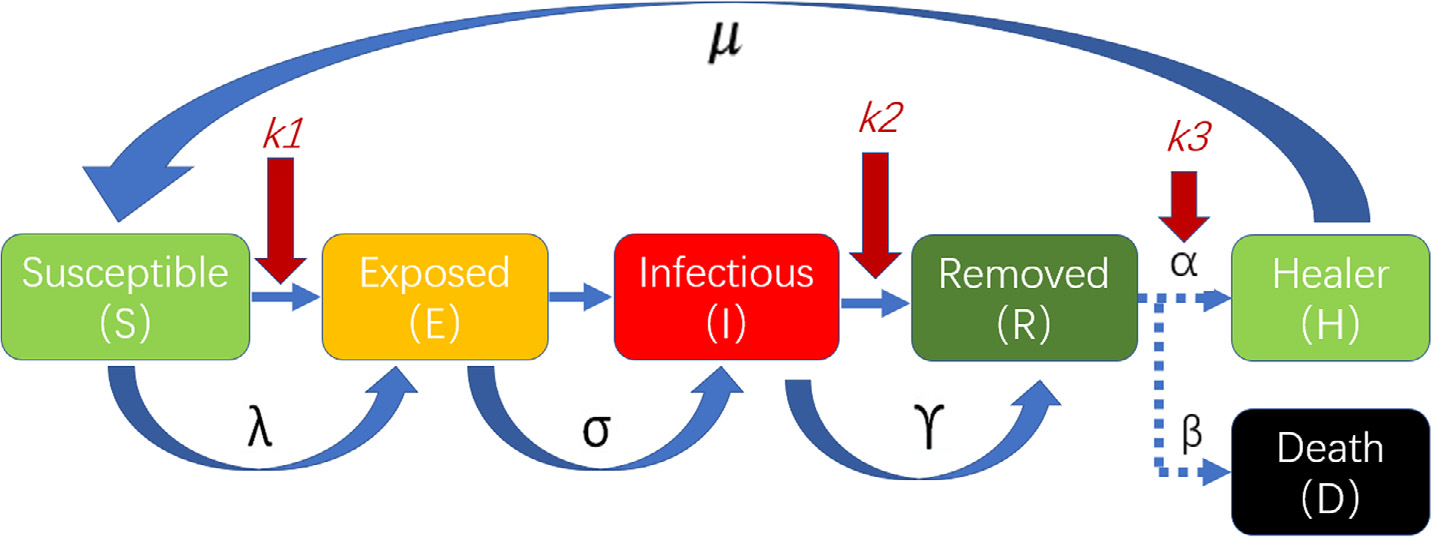
\includegraphics[width=\linewidth]{kseirscheme.png}
	\caption{Schemat działania modelu  \textit {K-SEIR}}
\end{figure}

Teoretyczny model K-SEIR został przekształcony w prosty oprogramowanie, zaimplementowane w języku PYTHON, przy użyciu inżynierii oprogramowania. W szczególności, ukończono zadania związane z projektowaniem interfejsu graficznego użytkownika, logiką sterowania, logiką operacji, kontrolą precyzji, kontrolą prędkości, wizualizacją danych, importem i eksportem danych, dopasowaniem parametrów, wyświetlaniem kluczowych danych oraz innymi konkretnymi treściami.
\newpage
\section{\textbf{Modele agentowe}}

Modele agentowe stanowią komputerowe symulacje, w których agenci, reprezentujący różne jednostki, mogą wejść w interakcję między sobą. Agentami mogą być jednostki takie jak osoby, organizacje, a nawet obszary geograficzne, takie jak województwa czy kraje. Wzajemne oddziaływania między agentami są określone przez zdefiniowane zasady programowe. Każdy z agentów podejmuje decyzje indywidualnie, co może obejmować zarówno proste wybory, na przykład decyzję o kierunku ruchu, jak i bardziej złożone decyzje, takie jak znalezienie konkretnego innego agenta lub sekwencję zdarzeń. W kontekście symulacji zarażeń, tego typu podejście pozwala na realistyczne uwzględnienie nieprzewidywalnych decyzji, jakie może podjąć jednostka.

Jednym z artykułów naukowych, poruszających temat modelowania agentowego pod tytułem: \textit{,,An open-data-driven agent-based model to simulate infectious disease outbreaks''} \cite{bib:artykul1} dostarczy nam cennych informacji na  temat implementacji takich rozwiązań. 

W artykule możemy przeczytać szczegółowe informacje na temat tego co badacze wzięli po uwagę podczas tworzenia swojego modelu.
był on oparty o dane populacji, umiejscowienia szkół i miejsc pracy a także danych dotyczących szczepień. Rzeczywiste dane są używane do określenia struktury wiekowej i płciowej naszych populacji, wraz z właściwym rozkładem wielkości gospodarstw domowych oraz innymi cechami takimi jak wiek dzieci. Następnie dane opisujące lokalizację szkół oraz miejsc pracy dają możliwość wiernego odwzorowania interakcji pomiędzy ludźmi. Na koniec aby ocenić podatność populacji na rozprzestrzenianie się choroby uwzględniono ilość szczepień (badanie opierało się na badaniu epidemii odry).
Następnym krokiem badaczy było wybranie testowanego obszaru i podzielenie go na mniejsze jednostki, w których przebywający ludzie są uznawani za mający kontakt ze sobą. Później należało rozmieścić agentów w odpowiednich domach według danych o populacji. Na koniec należało uwzględnić dodatkowe czynniki między innymi transport. 
Ostatnim krokiem było matematyczne opisane szans na zarażeniem, w tym celu autorzy wykorzystali równanie:

\begin{center}
$R_0 = cpd$
\end{center}

gdzie:\\
$R_0$ - prawdopodobieństwo infekcji. \\
$c$ - liczba kontaktów na jednostkę czasu. \\
$p$ - szansa na zarażenie podczas kontaktu. \\
$d$ - długość trwania infekcji \\

Poprzez przekształcenie równania otrzymano: 
\begin{center}
$ p = \frac{R_0}{cd} $
\end{center}

Dodatkowo w scenariuszach testowych, w których brano pod uwagę szczepienia użyto dodatkowego równania. Jest ono oparte na odporność zbiorowej jednak zmodyfikowane aby uwzględniać skuteczność szczepionki:

\begin{center}
	$V_c = \frac{(1-\frac{1}{R_0})}{V_e}$
\end{center}

gdzie:\\
$V_c$ - objęcie szczepieniami populacji \\
$V_e$ - skuteczność szczepionki. \\

Badacze przetestowali swój program na wielu miastach w Irlandii, ze względu na dostępne dane co do ich struktury oraz populacji.
Dodatkowo model został porównany z rzeczywistymi danych dotyczącymi epidemii odry w Schull, Irlandia w 2012 roku. Ze względu na losowość w modelu efekty każdej z symulacji było nieco inne. 

cyt. \textit{,, (...) Średnia liczba zainfekowanych agentów w różnych próbach wyniosła 17, przy maksymalnej liczbie 90 zainfekowanych agentów w jednym przypadku. Dwadzieścia pięć procent prób skończyło się wybuchem, w którym więcej niż 30 agentów zostało zainfekowanych. Wyniki pokazują, że chociaż średnia dla wszystkich prób jest niższa niż liczba zainfekowanych w przypadku wybuchu w Schull, to liczba faktycznie zainfekowanych osób znajduje się w 75. centylu wyników modelu.'' (...)}\cite{bib:artykul1}

Podsumowując, przewagą modeli agentowych nad modelami takimi jak SEIR jest uwzględnienie decyzji jednostki, przykładowo jeżeli mimo choroby osoba zdecyduje się pójść do szkoły lub pracy, ilość zarażeń wzrośnie lub odwrotnie jeżeli zdecyduje się zostać w domu, ilość zarażeń zmaleje, takie niuanse są wychwytywane dzięki skupieniu się na jednostce. Niestety takie podejście dużo gorzej radzi sobie w miarę zwiększania populacji, dlatego idealnie nadają się do symulacja epidemii w małych miastach ale nie w obrębie całego kraju lub świata.

\section{\textbf{Inne modele symulacji zarażeń}}

Ta część zwróci uwagę na dwie innowacyjne metody modelowania zarażeń, które stanowią wyjątkowe podejście w szerokim spektrum dostępnych metod. Ze względu na obecności różnorodnych podejść do modelowania zarażeń, skoncentrujemy się teraz na dwóch szczególnie interesujących metodach. Pierwszą z nich jest ambitny projekt symulacyjny oparty na algorytmach równoległych, korzystający z obszernych danych dotyczących populacji w Stanach Zjednoczonych. Drugą, równie pociągającą, jest aplikacja wykorzystująca technologię rozszerzonej rzeczywistości do wizualizacji, jak wirus może utrzymywać się na różnych powierzchniach i w konsekwencji jak może się szerzyć. Przechodząc do analizy tych dwóch wyjątkowych podejść w celu zidentyfikowania ich specyficznych zalet.

\subsection{\textbf{EpiSimdemics - równoległy algorytm symulacji epidemii}}
\textit{,,EpiSimdemics: an efficient algorithm for simulating the spread of infectious disease over large realistic social networks''} \cite{bib:konferencja} Jest bardzo ambitnym projektem wykorzystującym do obliczeń równoległy algorytm do symulowania rozprzestrzeniania się zarażeń w dużych i realistycznych symulowanych społeczeństwach. Badacze postanowili zasymulować niemalże statystycznie nierozróżnialną populację Stanów Zjednoczonych. Każdy z agentów w symulacji jest inny i opisany przez nawet do 163 zmiennych demograficznych z spisu ludności. Algorytm \textit{EpiSimdemics} opiera się na:
\begin{itemize}
	\item kolekcji jednostek z wartościami stanu i lokalnych reguł przejść między stanami
	\item grafie interakcji przechwytującego lokalną zależność jednostki od swoich sąsiednich jednostek
	\item sekwencji aktualizacji lub harmonogramu, takiego że związek przyczynowo-skutkowy w systemie jest 	reprezentowany przez składanie lokalnych odwzorowań
\end{itemize}
Z tych założeń są formułowane równania przejść stanów dla każdego z osobników w symulacji. Reprezentujące w jaki sposób stan wierzchołka (osobnika) i jego sąsiadujących wierzchołków będzie zmieniał się w trakcie trwania programu. Innymi słowy definiuje proces rozprzestrzeniania się choroby w siatce wierzchołków reprezentujących społeczeństwo.
	Dzięki zastosowaniu tak skomplikowanego systemu, program \textit{EpiSimdemics} posiada zdolność dostarczania szczegółowych informacji na temat rozprzestrzeniania się choroby w populacji, obejmujących takie detale jak konkretny zestaw osób zainfekowanych, miejsce zarażenia oraz kto ich zarażał.
\subsection{\textbf{Zastosowanie rozszerzonej rzeczywistości w symulacji zarażeń}}

Zainspirowani globalną pandemią COVID-19, badacze postanowili stworzyć innowacyjną aplikację pokazującą rozprzestrzenianie się wirusa poprzez różnego rodzaju powierzchnie i przedmioty, z którymi stykamy się w codziennym życiu. Udało się to dzięki wykorzystaniu rozszerzonej rzeczywistości, co pozwoliło na dokładne zobrazowanie, jak wirusy i bakterie mogą pozostawać na tych powierzchniach oraz jak łatwo mogą być przenoszone poprzez kontakty ręczne i inne interakcje. Aplikacja umożliwia użytkownikowi stworzenie własnego patogenu lub wybranie istniejącego, a następnie korzystając z kamery pozwala umieścić go w świecie wirtualnym. Użytkownik może śledzić, jak długo patogen utrzymuje się w danym miejscu, potencjalnie stanowiąc ryzyko przeniesienia się na inną osobę. Swoje spostrzeżenia i wnioski zawarli w artykule \textit{Bio-Virus Spread Simulation in Real 3D Space using Augmented Reality}\cite{bib:artykul2}

\begin{figure}[h!]
	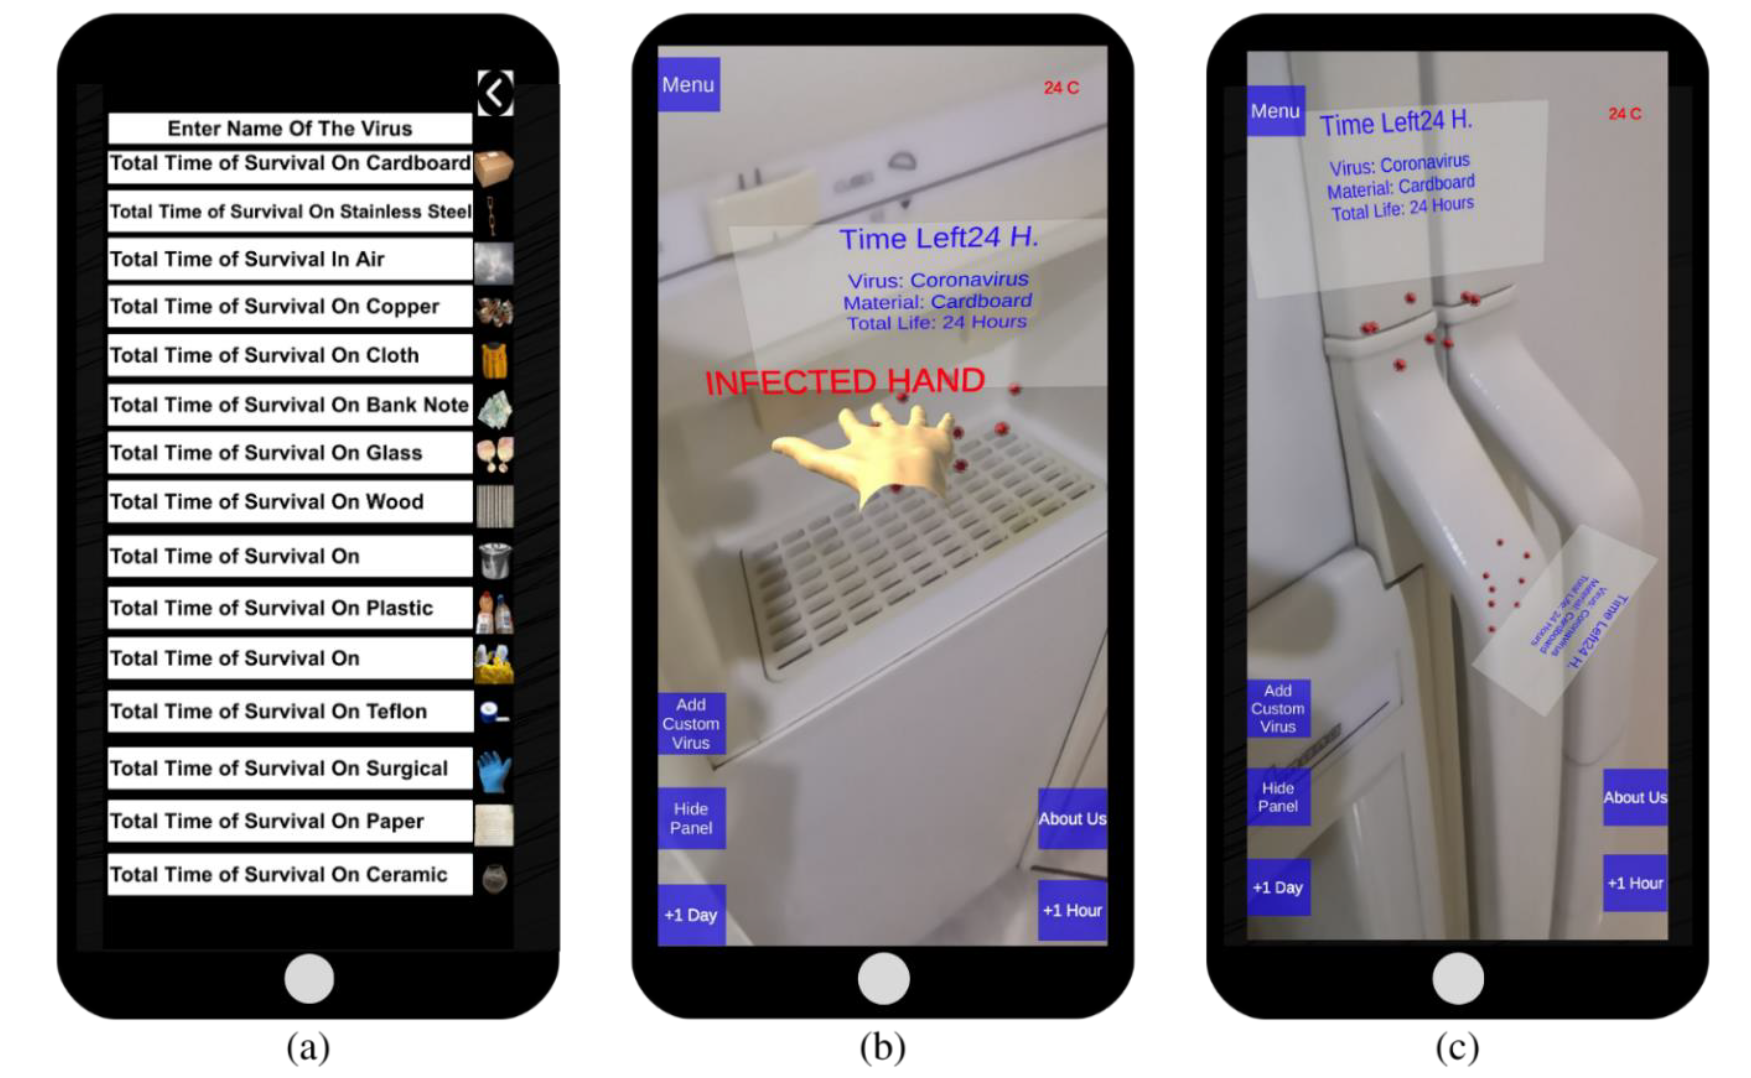
\includegraphics[width=\linewidth]{VirusIn3DSpaces.png}
	\caption{Demonstracja działania aplikacji: (a) dostosowywanie niestandardowego wirusa, (b) wprowadzenie wirusa w rzeczywistego świata, (c) wirus widoczny w rozszerzonej rzeczywistości z panelem informacyjnym.}
\end{figure}
%%%%%%%%%%%%%%%%%%%%%%%%



